\chapter{Neural network for nonlinear identification}
\section{Introduction}
In order to perform system identification for the linear systems, it is not necessary to use \textit{Neural Networks}. However, in the identification of the nonlinear systems, we deal with a much more challenging problem, which requires a more powerful techniques.\\

\section{Nonlinear system identification in a general setting}
Our aim is to identify a MIMO discrete-time dynamical system of input-output or regressor form:
\[
y_t = \mathcal{S}(y_{t-1},\, \cdots,\, y_{t-n},\,u_{t},\, \cdots, u_{t-n})
\]
where:
\(
\mathcal{S} : \underbrace{\mathbb{R}^p \times \cdots \times \mathbb{R}^p}_{\textcolor{blue}{n \text{ times}}}
\times \underbrace{\mathbb{R}^q \times \cdots \times \mathbb{R}^q}_{\textcolor{blue}{n+1 \text{ times}}}
\to \mathbb{R}^p
\) is a nonlinear function, and $y_t$ is the output.\\

This form for the linear systems becomes:
\[
y_t = \sum_{j = 1}^{n} \alpha_j y_{t-j} + \sum_{j = 0}^{n} \beta_j u_{t-j}
\]
We are given a set of experimentally collected input-output data.
\[
\{u_t,\,\tilde{y}_t\}_{t = 1}^{N}
\]
Different hypothesis on $\mathcal{S}$ are possible:
\begin{itemize}
    \item the structure of $\mathcal{S}$ is known from physical equations, and we want to estimate the physical parameters $\rightarrow$ \textbf{grey-box} identification, e.g. estimation of the magnetic constant of the system in a magnetic levitation problem.
    \item the structure of $\mathcal{S}$ is completely unknown $\rightarrow$ \textbf{black-box} identification.
    \item the structure is partially known from physical insights $\rightarrow$ \textbf{mixed grey-/black- box} identification; e.g. in the identification of a robotic system, from the physical insight, we will not have exponential terms of the position, it is possible that we have $\sin$ and $\cos$ functions and the prodoct of velocities, and so on.
\end{itemize}
\textbf{Neural networks are especially useful in black-box identification.}

\section{Introduction to Neural Netowrks}
A \textbf{Neural Netowrk}, NN, is the composition of functions called \textit{\textbf{layers}}.\\

Layer $\ell_i$ is a function $\mathbb{R}^{\nu_{i-1}} \rightarrow \mathbb{R}^{\nu_i}$ defined by:
\[
\alpha = \ell_i(x) = \Phi(W_ix + \beta_i)
\]
where,
\begin{itemize}
    \item $\nu_i$, the output dimension of the i-th layer, is also referred as \textbf{the number of neurons} of the i-th layer;
    \item $\alpha \in \mathbb{R}^{\nu_i}$ is the output of the layer;
    \item $x \in \mathbb{R}^{\nu_i -1}$ is the input of the layers;
    \item $W_i \in \mathbb{R}^{\nu_i \times \nu_{i-1}}$ is the weight matrix;
    \item $\beta_i \in \mathbb{R}^{\nu_i}$ is the bias vector;
    \item $\theta_i = [vec(W_i)^T,\,\beta_i^T]^T$ is called the \textbf{vector of parameters}
    \item $\Phi: \mathbb{R}^{\nu_i} \rightarrow \mathbb{R}^{\nu_i}$ is the activation function. It acts point-wise and in the same way on each entry of its input.
\end{itemize}
\begin{figure}[H]
    \centering 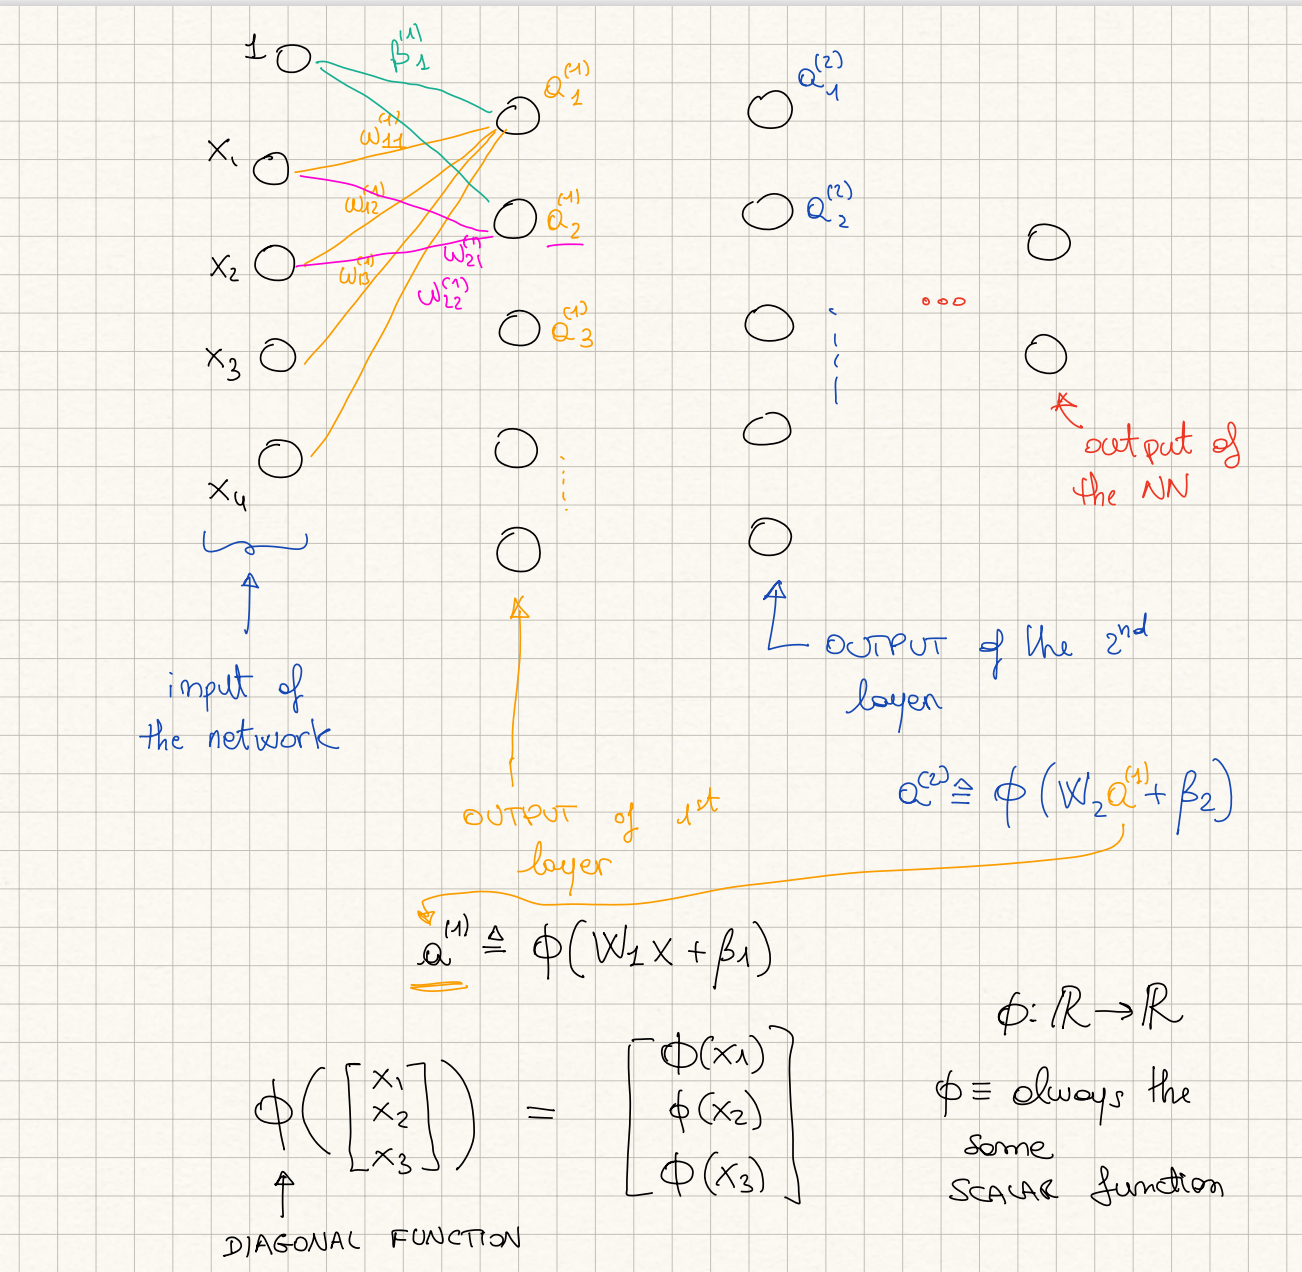
\includegraphics[width=0.75\textwidth]{sketch-of-nn.png}
    \caption{The scheme of a general neural network; pay attention that the bias is considered as an input node with the value 1 and the value of the bias for each input node is considered as the weight of that node.}
 \end{figure}

\textbf{typical activation functions} (for regression problem) are:
\begin{itemize}
    \item \textbf{Sigmoid}: 
    \[
    \sigma(z) = \frac{1}{1 + e^{-z}}
    \]
    \item \textbf{Hyperbolic Tangent} (tanh):
    \[
    \tanh(z) = \frac{e^z - e^{-z}}{e^z + e^{-z}}
    \]
    \item \textbf{ReLU} (Rectified Linear Unit)
    \[
    \text{ReLU} = \max(0\,z)
    \]
    \item \textbf{identity function} Typically used in the last layer to make the overall network's co-domain be $\mathbb{R}$.
\end{itemize}
\newpage

A\textbf{ \textit{single hidden layer ( or single-layer) neyral network} }is the function $\mathcal{N}:\:\mathbb{R}^{n_i} \rightarrow \mathbb{R}^{n_o}$
\[
z = \mathcal{N}(x) = \ell_2 ° \ell_1(x)
\]
selecting activation function \textit{ReLU} for the first layer and identify for the second, we get
\[
z = \mathcal{N}(x) = W_2 \text{ReLU}(W_1x + \beta_1) + \beta_2
\]
An \textit{\textbf{L-layer neural network}} is the function $\mathcal{N}:\: \mathbb{R}^{n_i} \rightarrow \mathbb{n_o}$,
\[
z = \mathcal{N}(x) = \ell_L \circ \ell_{L-1} \circ \cdots \circ \ell_2 \circ \ell_1(x) 
= W_L\phi(W_{L-1}\phi(\cdots \phi(W_2\phi(W_1x + \beta_1) + \beta_2) + \cdots) + \beta_{L-1}) + \beta_L
\]

\subsection{Universal Approximation Theorem; Barron, 1993}
Consider a single-layer neural network $\mathcal{N} : \mathbb{R}^{n_i} \to \mathbb{R}^{n_o}$ with $n$ neurons and $\tanh$ or $\sigma$ activation function. Let $\Omega \subset \mathbb{R}^{n_i}$ be a compact set. The approximation error of any function $f : \Omega \to \mathbb{R}^{n_o}$ can be bounded as:
\[
\|f - \mathcal{N}\|_{L^2} \doteq \left( \int_{\Omega} |f(x) - \mathcal{N}(x)|^2 \, dx \right)^{1/2} \leq \frac{C}{\sqrt{n}},
\]
where $C$ is a suitable constant dependent on the Fourier transform of $f$. The norm used here is the norm of $L^2$ in the \textit{Hilbert space}.\\

Variants o this theorem exists for \textbf{multi-layer networks} and \textbf{different activation functions}.\\

According to this theory, the more the number of neurons, the smaller error. The issue is that the number of neurons needed for a given class of functions is not known, thereby a trial and error is required for the network section.\\

When compared with linear approximators, e.g.,
\[
p = \sum\limits_{i} \theta_i p_i(x)
\]
where $p_(x)$ are polynomials (Weirestrass Theorem), the required number of parameters in the neural networks grows much less rapidly with the dimension of the problem, which is the dimension of the input space $n_i$!\\

\section{The NNARX model}
The first use of neural networks for system identificatino was to \textit{replace the unknown system function $\mathcal{S}$ with a neural network $\mathcal{N}$}. If the network is large enough and the parameters are properly selected: $\mathcal{N} \approx\mathcal{S}$

For the true system, \textbf{if the data are NOT affected by noise, we have}
\[
\begin{array}{c}
\tilde{y}_t = y_t \forall t
\tilde{y}_{n+1} = \mathcal{S}(\tilde{y}_n,\,\cdots,\,\tilde{y}_1,u_{n+1} ,\,\cdots,\,u_1) \\
\tilde{y}_{n+2} = \mathcal{S}(\tilde{y}_{n+1},\, \cdots,\,\tilde{y}_2,u_{n+2} ,\,\cdots,\,u_1) \\
\vdots \\
\tilde{y}_{N} = \mathcal{S}(\tilde{y}_{N-1},\,\cdots,\,\tilde{y}_N,u_N \,\cdots,\,u_{N-n}) \\
\end{array}
\]
which are a set of nonlinear equations with respect to the parameters of the neural network. However, up till now, even in the case of non-linear identification, we faced a problem that was linear with respect to the parameters.\\

Replacing $\mathcal{s}$ with $\mathcal{N}_\theta$, we get a system of equations in the parameters
\[
\theta \doteq [\text{vec}(W_1^T),\,\beta_1^T,\,\cdots,\, \text{vec}(W_L),\,\beta_L^T]
\]
Since these equations are nonlinear in the parameters, we cannot solve this problem. The combined effect of the mismatch between $\mathcal{S}$, $\mathcal{N}$, and the noise can be modelled as an equation error:
\[
\begin{array}{c}
\tilde{y}_t = y_t \forall t
\tilde{y}_{n+1} = \mathcal{N}_\theta(\tilde{y}_n,\,\cdots,\,\tilde{y}_1,u_{n+1} ,\,\cdots,\,u_1)  + e_{n+1}\\
\tilde{y}_{n+2} =\mathcal{N}_\theta(\tilde{y}_{n+1},\,\cdots,\,\tilde{y}_2,u_{n+2} ,\,\cdots,\,u_1)    + e_{n+2}\\
\vdots \\
\tilde{y}_{N} = \mathcal{N}_\theta(\tilde{y}_{N-1},\,\cdots,\,\tilde{y}_N,u_N ,\,\cdots,\,u_{N-n})    + e_{N} \\
\end{array}
\]
where the equation error $e_t$ is called \textbf{one-step ahead prediction error}.\\

To find the parameters, we formulate the following \textbf{nonlinear least square} optimization problem
\[
\arg \min\limits_{\theta} \sum\limits_{t=n+1}^{N} \|e_t\|_2^2 = \arg\min_{\theta} 
\underbrace{
\sum_{t=n+1}^{N} 
\left\| \tilde{y}_t - \mathcal{N}_{\theta}(\phi_t) \right\|_2^2
}_{\mathcal{L}(\theta)}
\]
where 
\[
\phi_t = [\tilde{y}_{t-1}^T,\,\cdots,\,\tilde{y}_{t-n}^T,\,u_t^T,\,\cdots,\,u_{t-n}^T]^T \in \mathbb{R}^{n_i},\:\:\:\:\:\:\: n_i \doteq pn + (n\,+\,1)q
\]
is the regressor vector.\\
The optimization problem here is non-convex, and high-dimensional. It's usually solved, or \textit{"trained"} using a \textbf{gradient algorithm}, e.g. gradient descent.
\[
\theta \gets \theta - \alpha \nabla_{\theta} \mathcal{L}(\theta), \quad \alpha > 0
\]

\begin{factbox}[Clarification]
In the context of neural networks, the term \textbf{training} is equivalent to identifying the model, or estimating the parameters.\\

In the formula for updating the value of the $theta$ in an iterative fashion, the idea is that if the slope is negative, it means that by increasing the value of the $theta$ the value of $\mathcal{L}(\theta)$ reduced, and vice versa, thereby getting closer to a local minimum. Therefore, whether we reach the global minimum depends on the initial point, since there is  always the risk of trapping in a local minimum.
\end{factbox}

In general, o\textbf{nly a local minima can be found.} Different runs with different initial conditions lead to different results. 

\subsection{Prediction vs. Simulation}
\textbf{Since we minimize the one-step-ahead prediction error (equation error), the resulting network is usually good at one-step prediction but exhibits very low performance in simulation.} In the simulation models, the predicted output is fed as an input for predicting the next step rather than the measured data.\\

\begin{figure}[H]
    \centering 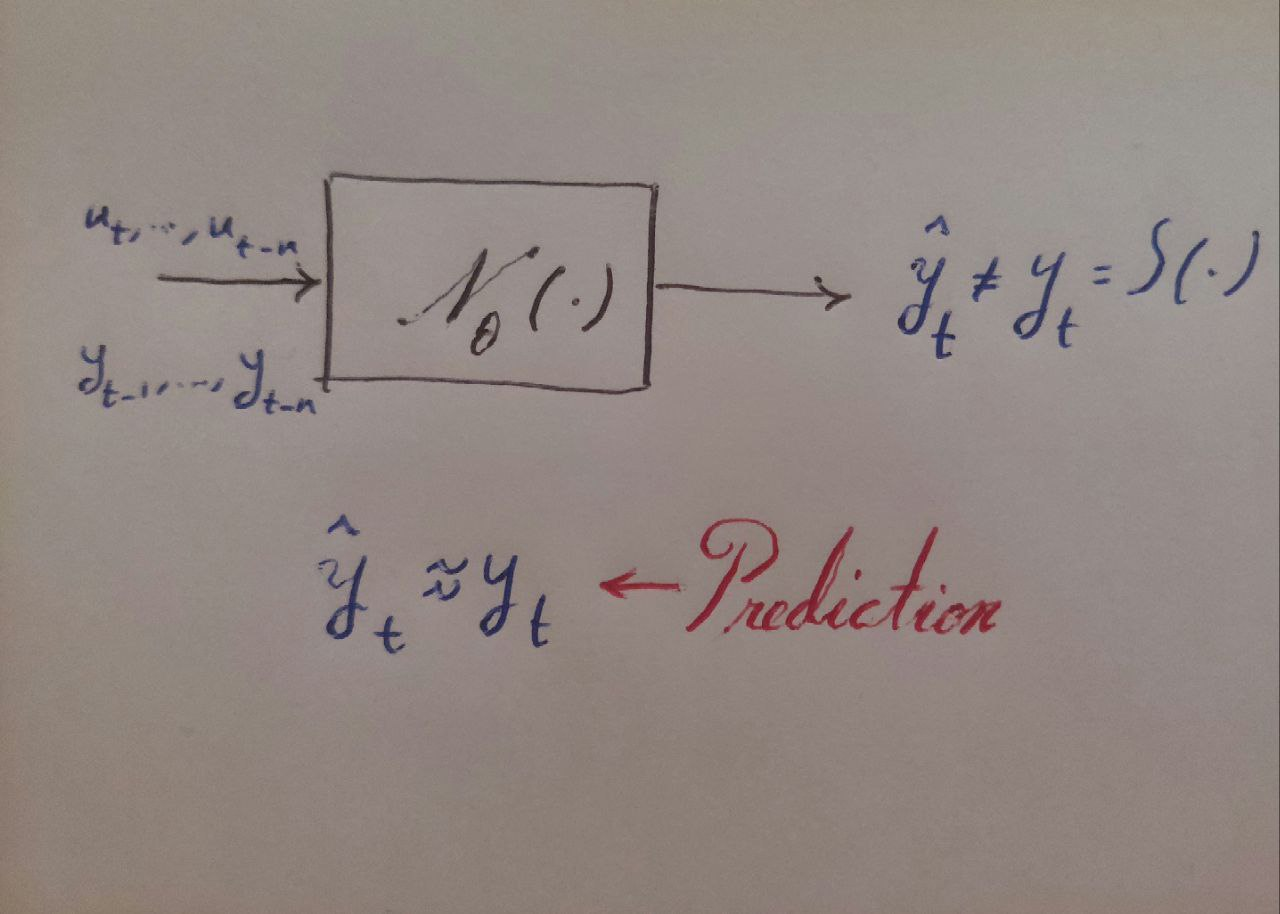
\includegraphics[width=0.5\textwidth]{prediction.jpg}
    \caption{Blockdiagram representation of the prediction problem.}
 \end{figure}

\begin{figure}[H]
    \centering 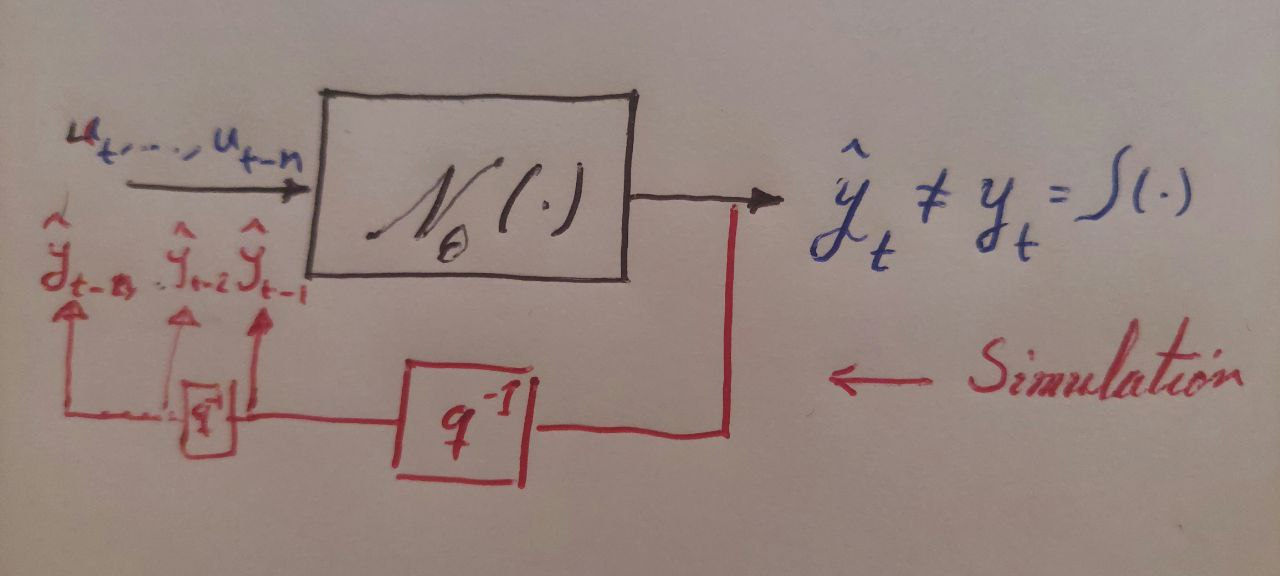
\includegraphics[width=0.5\textwidth]{simulation.jpg}
    \caption{Blockdiagram representation of the simulation problem.}
 \end{figure}

\section{Recurrent Neural Netowrks}
\textbf{NNARX} are \textbf{static neural networks }taking as input the regressor. To get good simulation performances, we must consider the dynamics during the identification. By definition, \textbf{dynamic neural networks} are the networks which can approximate any dynamical system. Neural networks which contain dynamics in their definition are called \textbf{reccurent networks (RNNs)}. Several types of them, some of which will be discussed in this seciton.

\subsection{Elman RNN}
Introduced in 1990, each layer $i$ of the Elman RNN is a nonlinear state-space model with state $h^{(i)}$ of the kind:
\[
h_t^{(i)} = \phi(W_ix_t^{(i)} + V_ih_{t-1}^{(i)} + \beta_i)
\]
where $h_t^{(i)} $ is the output or the state, $x_t^{(i)}$ is the input to the layer, $V_ih_{t-1}^{(i)} $  linear combination of the previous states. \\
The first layer takes as input $x$ the input of the system $u$. Starting from the second layer, each layer takes the state of the previous ones as input:
\[
x_t^{(i)} = h_t^{i-1}
\]
The last layer defines the output . It is generally static and uses identity activation.
\[
y_t = W_Lh_t^{L-1} + \beta_L
\]
\begin{figure}[H]
    \centering 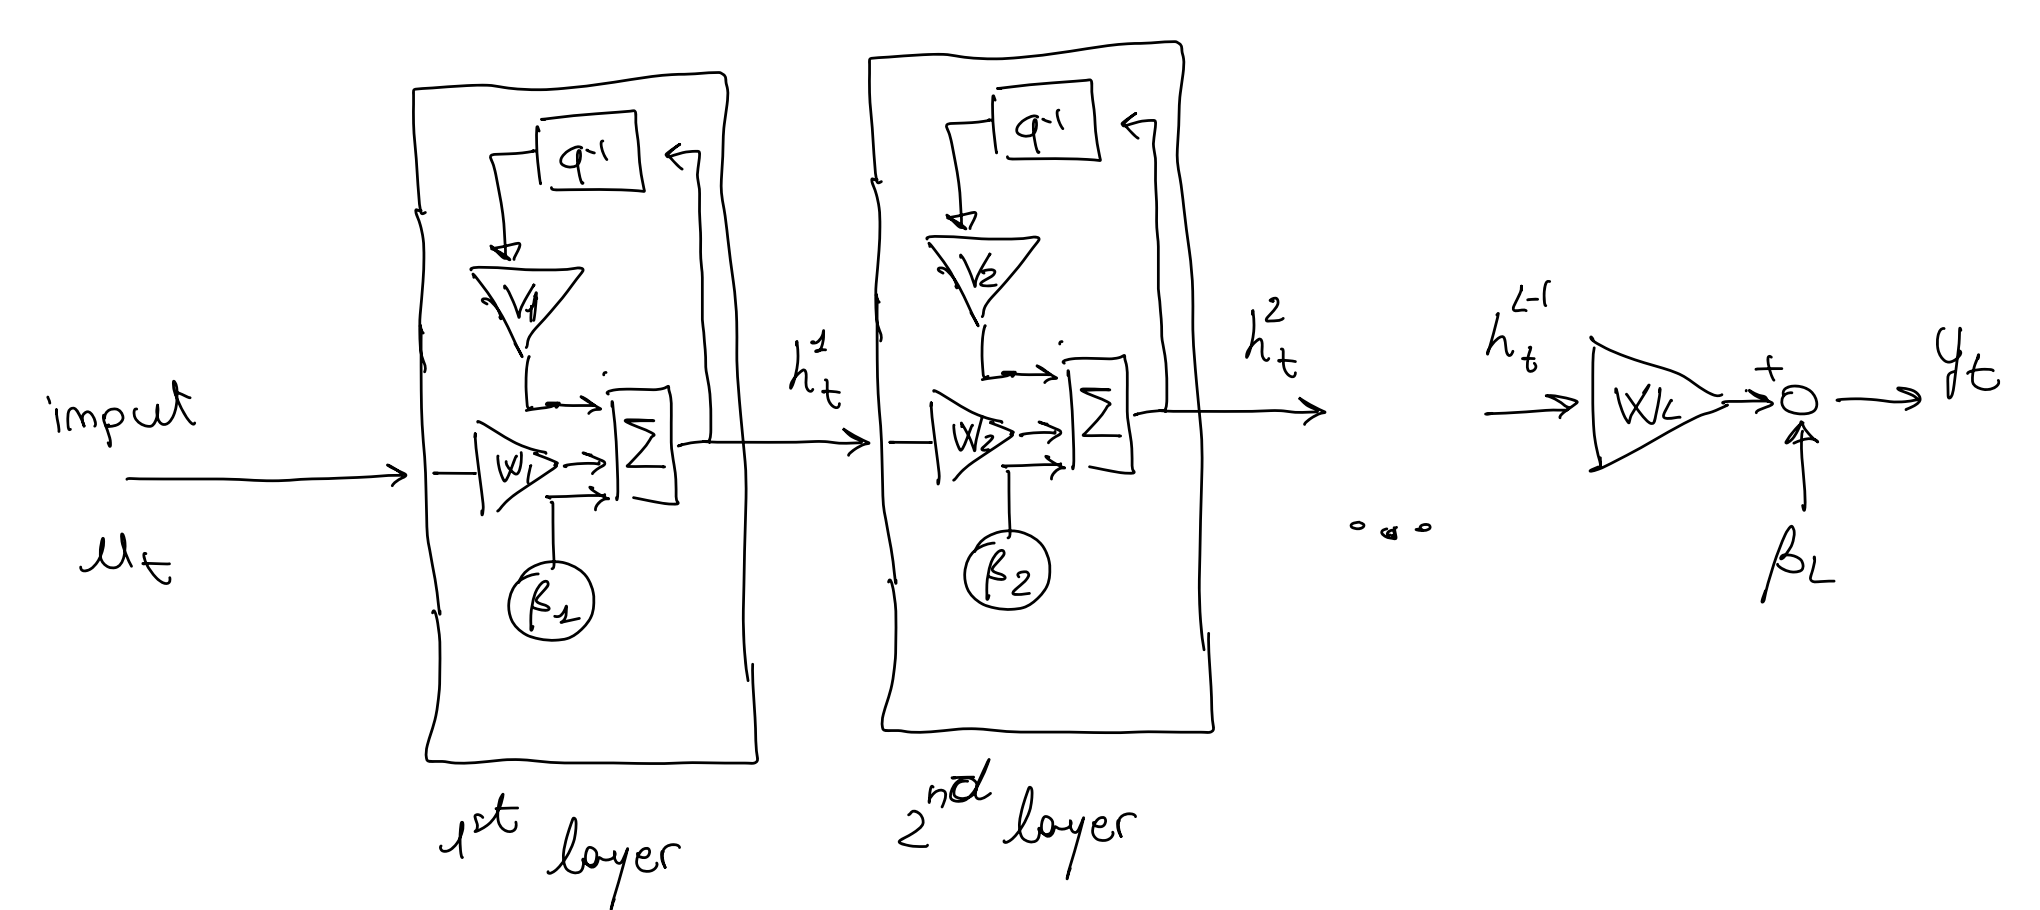
\includegraphics[width=0.5\textwidth]{elman-rnn.png}
    \caption{The blockdiagram representation of Elman RNN}
 \end{figure}

\subsection{Neural state-space models}
Use stsatic neural networks $\mathcal{N}_f$, $\mathcal{N}_h$ to approximate the unknown function in a state-space representation of the system
\[
x_{t+1} = \mathcal{N}_f([u_t^T,x_t^T]^T)
\]
\[
y_t = \mathcal{N}_h([u_t^T,x_t^T]^T)
\]
$\mathcal{N}_f$, and $\mathcal{N}_h$ can have an arbitrary number of layers and number of neurons per layer.

\begin{figure}[H]
    \centering 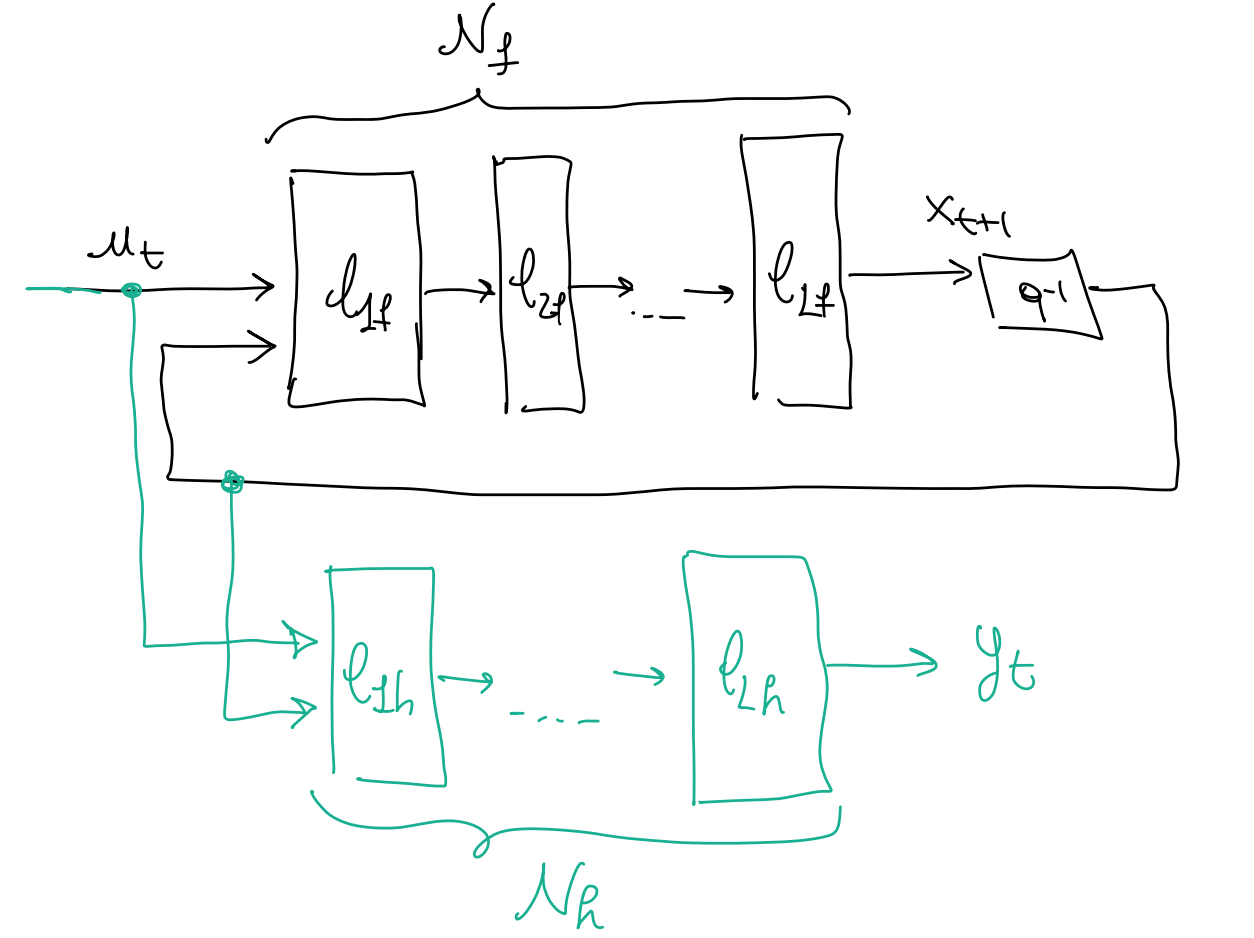
\includegraphics[width=0.5\textwidth]{neural-state-space.png}
    \caption{The blockdiagram representation of Neural state-space models.}
 \end{figure}

\subsection{NNOE model}
Defined by the recursive equation, it is the dynamic counterpart of the NNARX network.
\[
y_t = \mathcal{N}([y_{t-1}^T,\,\cdots,\,y_{t-n}^T,\, u_{t}^T,\, u_{t-n}^T])
\]
Differentlly from the NNARX model, this network takes as input a regressor \textbf{built using its own previously generated outputs, not the noisy measured ones, meaning that it should be used recursively!} This is what we discussed as the simulation of the system.


\begin{figure}[H]
    \centering 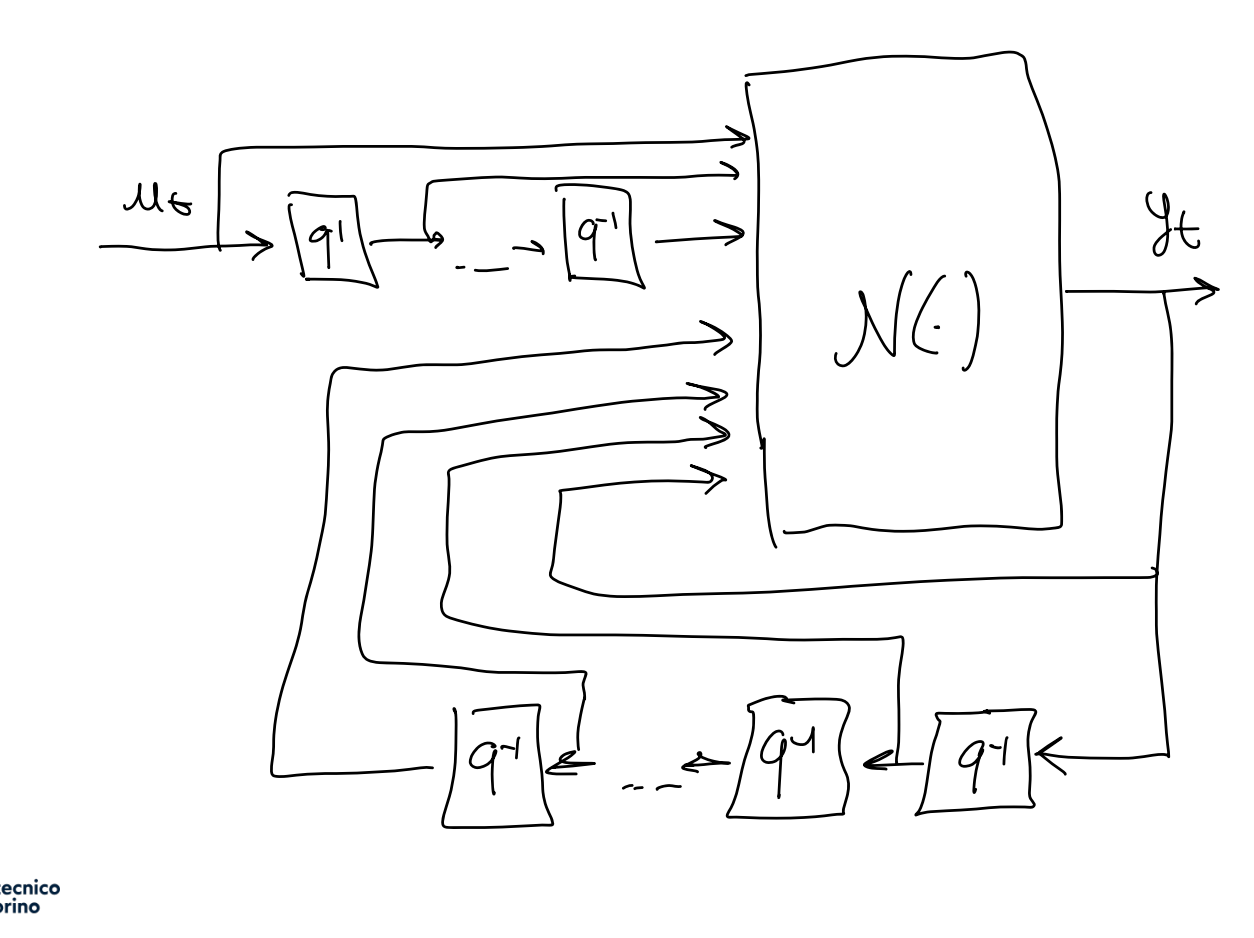
\includegraphics[width=0.5\textwidth]{NNOE.png}
    \caption{The blockdiagram representation of NNOE.}
 \end{figure}

\subsection{Identification of RNNs}
To identify the RNN models, we look for parameters that minimize the difference between the \textbf{measured output } and \textbf{the output produced by the model.} In formulae, we define the optimization problem
\[
\theta  = \arg\min\limits_{\theta} 
\underbrace{
\sum_{t=1}^{N} \|\tilde{y}_t -\hat{y}_t(u_t,x_0)\|_2^2}_{\mathcal{L}(\theta)}
\]
$\hat{y}_t(u_t,\,x_0)$ is the output of the RNN given the (measured) input $u_t$ and initial condition $x_0$ (usually assumed zero or random). It is a strongly nonlinear function of the RNN parameters.\\

The optimization problem, like before, is solved using some gradient-descent algorithm, in case of a SISO system:
\[
\theta \gets \theta - \alpha 2 \underbrace{\sum\limits_{t=1}^{N}(\tilde{y}_t - \hat{y}_t(u_t,\,x_0))\nabla_\theta\hat{y}_t(u_t,\,x_0)}_{\nabla_\theta \mathcal{\theta}}
\]
Due to the dynamic nature of the problem, the gradients $\nabla_\theta \hat{y}_t$ are related to each other, meaning that $\nabla_\theta \hat{y}_t$ depends on $\nabla_\theta \hat{y}_{t-1}$, $\nabla_\theta \hat{y}_{t-2}$, and so on. The relation between $\nabla_\theta \hat{y}_t$ at different time samples \textbf{implicitly define a dynamical system the output of which are the gradients}.

\subsection{Vanishing and exploding gradient issues}
If such a system is stable, as $t \to \infty$, the gradients vanish (even if it is not a local minimum), which is called \textbf{vanishing gradient issue.} If such a system is unstable, however, as $t \to \infty$, the gradients vanish (diverge), which is called \textbf{exploding gradient issue}. 

\begin{example}
For example, consider an NNOE network with zero layers and identity activation function, or a neural state-space model of order 1 and $y_t = x_t$.  
\[
y_t = \alpha y_{t-1} + \beta u_{t-1}
\]  
recursively propagates outputs, and the gradient of the loss \(L\) with respect to \(\alpha\) is:  
\[
\frac{\partial L}{\partial \alpha} = \frac{\partial L}{\partial y_t} \cdot \frac{\partial y_t}{\partial \alpha}.
\]

The dependency of \(y_t\) on \(\alpha\) involves terms like \(\alpha^{t-1}\), leading to two phenomena:

1. **Gradient Vanishing** (\(|\alpha| < 1\)):  
   \[
   \alpha^{t-1} \to 0 \quad \text{as} \quad t \to \infty.
   \]
   Gradients for earlier time steps become negligible, making it hard to learn long-term dependencies.

2. **Gradient Exploding** (\(|\alpha| > 1\)):  
   \[
   \alpha^{t-1} \to \infty \quad \text{as} \quad t \to \infty.
   \]
   Gradients grow excessively, causing instability during training.
\end{example}
\begin{example}
**Mitigation Strategies**:  \\
- **Gradient Clipping**: Limit \(\frac{\partial L}{\partial \alpha}\) to prevent large updates.  \\
- **Regularization**: Penalize large \(|\alpha|\) in the loss function.\\  
- **Advanced Architectures**: Use LSTMs/GRUs to manage long-term dependencies.\\  
- **Proper Initialization**: Start \(\alpha\) near 1 to avoid extreme behaviors.  
\end{example}
Following solutions are introduced for resolving these problems.

\subsection{Long Short-Term Memory (LSTM)}
LSTMs address the vanishing gradient problem by introducing a \textbf{direct propagation path} for the gradient. It consists of three gates: forget, input, and output, which in turn shape a layer:
\[
\begin{cases}
f_t = \sigma(W_f[h_{t-1},\,x_t] + b_f), \\
i_t = \sigma(W_i[h_{t-1},\,x_t] + b_i), \\
o_t = \sigma(W_o[h_{t-1},\,x_t] + b_o), \\
\tilde{c}_t = \tanh(W_c[h_{t-1},\,x_t] + b_c), \\
\textcolor{red}{c_t = f_t c_{t-1}} + i_t \tilde{c}_t, \\
h_t = o_t \tanh(c_t).
\end{cases}
\]
The red part of the formula represents the direct propagation of the state, which helps mitigate the vanishing and exploding gradient issues.

\subsection{Gated Recurrent Unit (GRU)}
This method combines the forget and input gates into a single update gate, simplifying the architecture compared to LSTM:
\[
\begin{cases}
z_t = \sigma(W_z[h_{t-1},\,x_t] + b_z), \\
r_t = \sigma(W_r[h_{t-1},\,x_t] + b_r), \\
\tilde{h}_t = \tanh(W[r_t ,\, h_{t-1},\,x_t] + b), \\
\textcolor{red}{h_t = (1 - z_t) h_{t-1} + z_t \tilde{h}_t}.
\end{cases}
\]

\subsection{Beyond LSTM and GRU}
LSTM and GRU architectures are designed to attenuate the vanishing gradient problem but do not fully solve it.  
They require significantly more parameters than standard RNNs (e.g., Elman, neural state-space, and NNOE models). Consequently, they need more data and computational effort to perform identification.  

Improvements to LSTM and GRU exist. For instance, mini-LSTM and mini-GRU (Feng et al., 2024) reduce the number of parameters and better exploit GPUs for computations, although the vanishing gradient problem still persists.  

Transformers (Vaswani et al., 2017) are generally considered a superior alternative to RNNs. GPT models are based on this architecture and are particularly suited for processing text sequences. However, their application in system identification is limited due to their complexity and lack of intrinsic dynamics.

\section{Modern Trends}

A new approach to eliminating the vanishing and exploding gradient problems is based on avoiding the calculation of \(\nabla_\theta \hat{y}_t\). This is possible if we formulate the identification problem as a \textbf{constrained optimization} problem:
\[
\hat{\theta} = \arg \min\limits_{\theta,\,y} \sum\limits_{t=1}^{N} \|\tilde{y}_t - y_t\|_2^2 
\quad \text{s.t.} \quad y_t = \mathcal{N}_\theta(y_{t-1},\,\cdots,\,y_{t-n},\,u_t,\,\cdots,\,u_{t-n}), \quad \forall t = 1,\,\cdots,\,N.
\]

For the case of the NNOE model, the resulting problem is more challenging computationally because it is constrained and has more variables.

We solve this problem using a first-order constrained optimization algorithm, designed by leveraging feedback control system theory. The resulting identification algorithm is faster and more accurate than LSTM and GRU for a wide range of medium-size identification problems. Current research efforts focus on improving the scalability of the method for large-scale problems.









